\documentclass{article}

\usepackage[margin=0.5in]{geometry}
\usepackage{multicol}
\usepackage{siunitx}
\usepackage{tikz}
\usepackage{amsthm}

\title{Solid Geometry Lecture Problems}
\author{}
\date{}

\begin{document}
\maketitle

\begin{enumerate}
    \item In the figure shown, a triangular pyramid has been cut off the corner of the cube so that an equilateral triangle face is formed.
        If each corner of the cube is cut off in this manner, what is the maximum sum of the number of faces, edges, and vertices on the new polyhedron?
        \begin{center}
            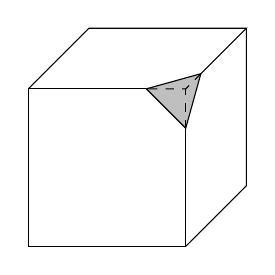
\begin{tikzpicture}[scale=0.5]
                \draw (3,4,4) -- (0,4,4) -- (0,0,4) -- (4,0,4) -- (4,3,4);
                \draw (0,4,4) -- (0,4,0) -- (4,4,0) -- (4,4,3);
                \draw (4,4,0) -- (4,0,0) -- (4,0,4);
                \draw[fill=lightgray] (4,4,3) -- (3,4,4) -- (4,3,4) -- cycle;
                \draw[dashed] (4,4,3) -- (4,4,4) -- (3,4,4);
                \draw[dashed] (4,3,4) -- (4,4,4);
            \end{tikzpicture}
        \end{center}
    \vspace{0.5cm}
    \item What is the number of solid $3$-inch by $2$-inch by $2$-inch rectangular prisms that can be arranged to form a solid cube of edge length $1$ foot?
        \vspace{3cm}
    \item Keaton wants to build a rectangular prism with volume $\SI{2016}{in^2}$ so that the length of each edge is a whole number of inches.
        What is the least possible sum of the three dimensions of the prism he builds?
    \vspace{3cm}
    \item When a cone's height is decreased by a factor of four, to maintain the same volume, the radius must be increased by a factor of two, or $100\%$.
        When the cone's height is decreased by a factor of three, by what percent must the radius be increased to maintain the same volume?
        Express your answer to the nearest whole number.
    \vspace{3cm}
    \item A sphere is inscribed in a cube.
        What is the ratio of the volume of the cube to that of the sphere?
        Express your answer as a common fraction in terms of $\pi$.
\vspace{3cm}
\end{enumerate}
\end{document}
